%%%%%%%%%%%%%%%%%%%%%%%%%%%%%%%%%%%%%%%%%%%%%%%%%%%%%%%
% % Lines starting with % are comments, which are ignored.
% % This is a handy way of indicating the date and version of
% % your document, to wit:
% %
% % LaTeX sample file
% % Modified March, 2002
% %
%%%%%%%%%%%%%%%%%%%%%%%%%%%%%%%%%%%%%%%%%%%%%%%%%%%%%%%
\DocumentMetadata{
  % PDF standards: ONE key whose value is a comma-separated list --
  % UA-2 (accessibility) plus A-4f (archival; the archival companion of
  % UA-2). Do NOT use separate pdfstandard=... keys: with ordinary
  % key-value parsing only the last one takes effect.
  pdfstandard={UA-2,A-4f},
  lang=en-US,
  tagging=on,
  tagging-setup={
    math/setup=mathml-SE
  }
}

\documentclass[12pt]{exam}
% worksheet-macros.tex -- shared package setup for worksheet-template.tex.
%
% NOTE ON PATHS: every template in this repository is stored one level up
% from where it is compiled (see README.md). All relative \input paths
% below are resolved against the folder the document is compiled in,
% which sits one directory above this file.

% --- Math ------------------------------------------------------------
% amsmath: equation environments and numbering
% amsfonts: \mathbb etc.  |  mathrsfs: \mathfrak  |  stmaryrd: extra symbols
\usepackage{amsmath}
\usepackage{amsfonts}
\usepackage{mathrsfs}
\usepackage{stmaryrd}

% --- Layout and glyphs ------------------------------------------------
% float: [H] float placement (stop floats where you put them)
% fontspec: Unicode/OpenType fonts (compile with XeLaTeX or LuaLaTeX)
% emoji: emoji glyphs in the text
\usepackage{float}
\usepackage{fontspec}
\usepackage{emoji}

% --- Typography --------------------------------------------------------
% Atkinson Hyperlegible as the document-wide sans serif (sfdefault):
% a high-legibility face that is easier to read for students with
% dyslexia or low vision.
\usepackage[sfdefault]{atkinson}

% --- Colors -------------------------------------------------------------
% dvipsnames: extended named color palette (the Accessible* colors in
%   lecture-macros.tex are built on it);
% table: \rowcolors / \cellcolor for shading worksheet tables.
% NOTE: xcolor may only be loaded ONCE per document -- a second
% \usepackage{xcolor} with different options is a fatal "Option clash"
% error, so ALL of its options are listed here.
\usepackage[dvipsnames,table]{xcolor}

% --- Multimedia ---------------------------------------------------------
% animate: embeds audio/video (and legacy Flash) media in the worksheet.
\usepackage{animate}

% --- Bibliography --------------------------------------------------------
% biblatex (biber backend): citations and a reference list for worksheets.
\usepackage[
  backend=biber,
  style=alphabetic,
  url=true,
  doi=true,
  isbn=true,
  backref=true
]{biblatex}

% --- Links ---------------------------------------------------------------
% hyperref makes every \ref/citation/URL clickable in the PDF.
% Link colors must satisfy WCAG 1.4.3 (>= 4.5:1 contrast on white):
%   blue = 8.6:1, green!40!black = 7.2:1.
% (The old cyan/magenta values measured 1.25:1 / 3.1:1 and failed.)
\usepackage{hyperref}
\hypersetup{
  colorlinks=true,
  linkcolor=blue,
  filecolor=blue,
  urlcolor=green!40!black,
}

% --- Shared course macros ------------------------------------------------
% Root macros.tex: math shorthands used across all course documents
% (\RR, \NN, \ZZ, \QQ, \grad, \curl, \tr, \der, \pder, ...).
\newcommand{\RR}{\mathbb{R}}
\newcommand{\NN}{\mathbb{N}}
\newcommand{\ZZ}{\mathbb{Z}}
\newcommand{\QQ}{\mathbb{Q}}
\newcommand{\vv}{\vec{v}}
\newcommand{\ww}{\vec{w}}
\newcommand{\xx}{\vec{x}}
\newcommand{\yy}{\vec{y}}
\newcommand{\zz}{\vec{z}}
\newcommand{\uu}{\vec{u}}
\newcommand{\basis}[1]{\vec{e_{#1}}}
\newcommand{\id}{\mathrm{id}}
\newcommand{\CC}{\mathbb{C}}
\renewcommand{\div}{\operatorname{div}}
\newcommand{\grad}{\operatorname{grad}}
\newcommand{\curl}{\operatorname{curl}}
\newcommand{\tr}{\operatorname{tr}}
\newcommand{\der}[2]{\dfrac{d #1}{d #2}}
\newcommand{\pder}[3][]{\dfrac{\partial^{#1} #2}{\partial #3}}


% % Title and author(s)
%%%%%%%%%%%%%%%%%%%%%%%%%%%%%%%%%%%%%%%%%%%%%%%%%%%%%%%
\title{Worksheet 15: Optimization I}
\author{MATH 1271}
\date{10/29/2026}
%%%%%%%%%%%%%%%%%%%%%%%%%%%%%%%%%%%%%%%%%%%%%%%%%%%%%%%
% %
% % The next command allows your in import encapsulated
% % postscript files, .epsf or .eps files, which
% % contain vector graphic image data.
% %
%%%%%%%%%%%%%%%%%%%%%%%%%%%%%%%%%%%%%%%%%%%%%%%%%%%%%%%
% %   The first thanks indicates your affiliation
% %
% %  Just the name here.
% %
% % Your mailing address goes at the end.
% %
% % \thanks is also how you indicate grant support
% %
%%%%%%%%%%%%%%%%%%%%%%%%%%%%%%%%%%%%%%%%%%%%%%%%%%%%%%%

%%%%%%%%%%%%%%%%%%%%%%%%%%%%%%%%%%%%%%%%%%%%%%%%%%%%%%%
% $ The next command ensures the margins are 1 inch on
% % all sides.
% %
%%%%%%%%%%%%%%%%%%%%%%%%%%%%%%%%%%%%%%%%%%%%%%%%%%%%%%%
\begin{document}
\newpage
\maketitle

\begin{enumerate}

\item Suppose that $g(x)$ is a function that is continuous at every value of $x$ except at $x=2$. You may assume that this is because $g$ has a vertical asymptote at $x=2$. 

You may also assume that the \textbf{first derivative} of $g$ is
$$g'(x)=\dfrac{(x+4)(x-1)^2}{(x-2)}$$

\begin{enumerate}

\item Determine all critical numbers of $g$.

\vspace{2.5in}

\item By developing a carefully labeled first derivative sign chart, decide whether $g$ has a local minimum, local maximum, or neither at each critical number.

\vfill

\newpage

\item Which of the following graphs is a possible graph of $y=g(x)$?

\bigskip

\begin{enumerate}

\item \; 

\vspace{-25pt} 

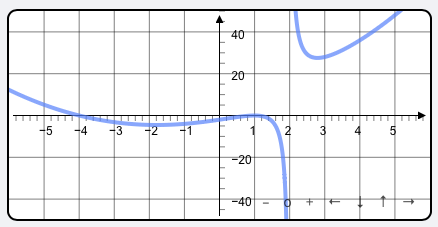
\includegraphics[scale=0.65]{wkst16option1-f25}

\bigskip

\item \; 

\vspace{-25pt} 

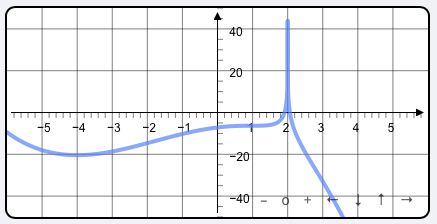
\includegraphics[scale=0.65]{wkst16option2-f25}

\bigskip

\item \; 

\vspace{-25pt} 

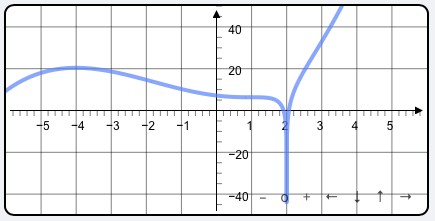
\includegraphics[scale=0.65]{wkst16option3-f25}

\bigskip

\item \; 

\vspace{-25pt} 

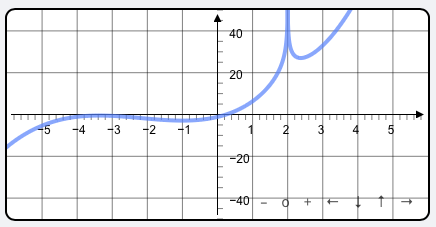
\includegraphics[scale=0.65]{wkst16option4-f25}

\end{enumerate}

\end{enumerate}

\bigskip

\newpage



\item 

\begin{enumerate}

\item Let $f(x)=x^4(x-1)^3$. 

\begin{enumerate}

\item The function $f$ has three critical numbers; find them. 

\vfill

\item You may assume that
$$f''(x)=6x^2(x-1)(7x^2-8x+2)$$
What does the Second Derivative Test tell you about the critical numbers you found in part (a)?

\vfill

\item What does the First Derivative Test tell you about the critical numbers you found in part (a)?

\vfill

\end{enumerate}

\newpage

\item Let $g(t)=t^2\ln(t)$. 

\begin{enumerate}

\item The function $g$ has one critical number; what is it?

\vfill

\item Is this critical number a local maximum of $g$, a local minimum of $g$, or neither one?

\vfill

\end{enumerate}

\end{enumerate}

\newpage


\item Suppose that $g$ is a function whose \textbf{second derivative}, $g''$, is given by the graph below:

\begin{center}
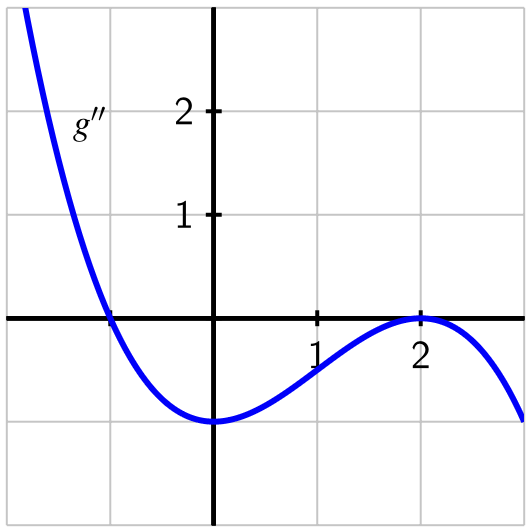
\includegraphics[scale=0.3]{wkst16graph-f25}
\end{center}

\begin{enumerate}

\item Find the $x$-coordinates of all points of inflection of $g$.

\vfill

\item Suppose you are given that $g'(-1.67857351)=0$. Is there a local maximum, local minimum, or neither (for the function $g$) at this critical point, or is it impossible to say?

\vfill

\item Assuming that $g''(x)$ is a polynomial (and that all important behavior of $g''(x)$ is seen in the graph above), what degree polynomial do you think $g(x)$ is? (Hint: Think about the Power Rule. How does the degree of a polynomial relate to the degree of its second derivative?)

\vfill

\end{enumerate}

\end{enumerate}


% Most people don't use these, so they are "commented out"
% by starting the lines with a "%"
%\begin{keywords}
%   \LaTeX, typesetting
%\end{keywords}

%\begin{AMS}
%   50C60, 18C25
%\end{AMS}

%%%%%%%%%%%%%%%%%%%%%%
% % Here is the start of the Text
%%%%%%%%%%%%%%%%%%%%%%
\end{document}
